\subsection{Deleting an Existing Account}

This screen consists of a confirmation alert dialog, activated whenever an account is about to be deleted. Deleting an account will delete all transactions related to the account, and it is an action that cannot be undone. Hence, this alert dialog exists to confirm the action.

\subsubsection{Application Screenshots}
\begin{figure}[h]
 
\begin{subfigure}{0.5\textwidth}
  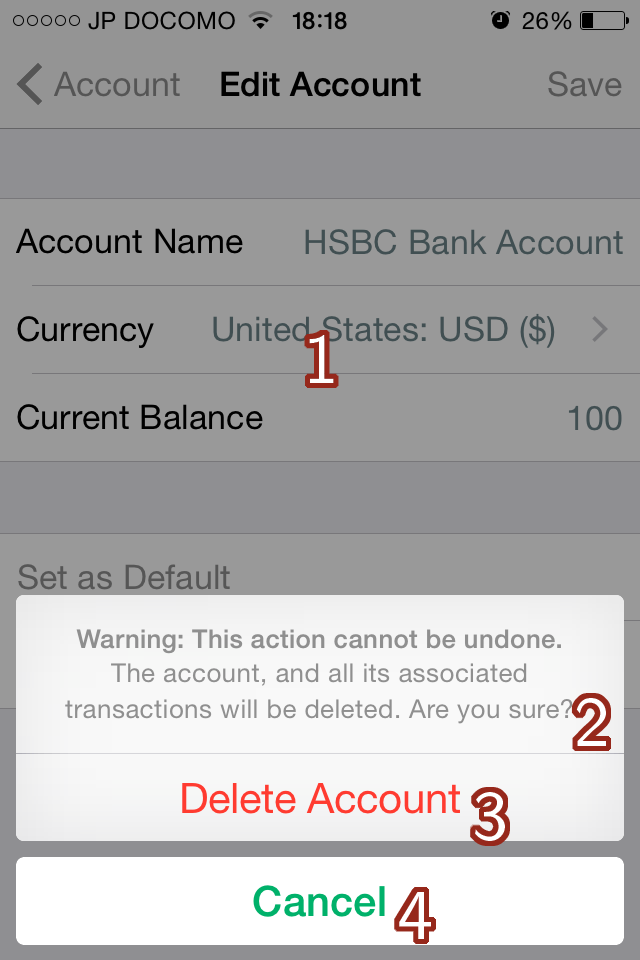
\includegraphics[scale=0.35]{ACC-0003-3} 
  \caption{Deleting from Edit Account}
  \label{fig:delete-account-1}
\end{subfigure}
\begin{subfigure}{0.5\textwidth}
  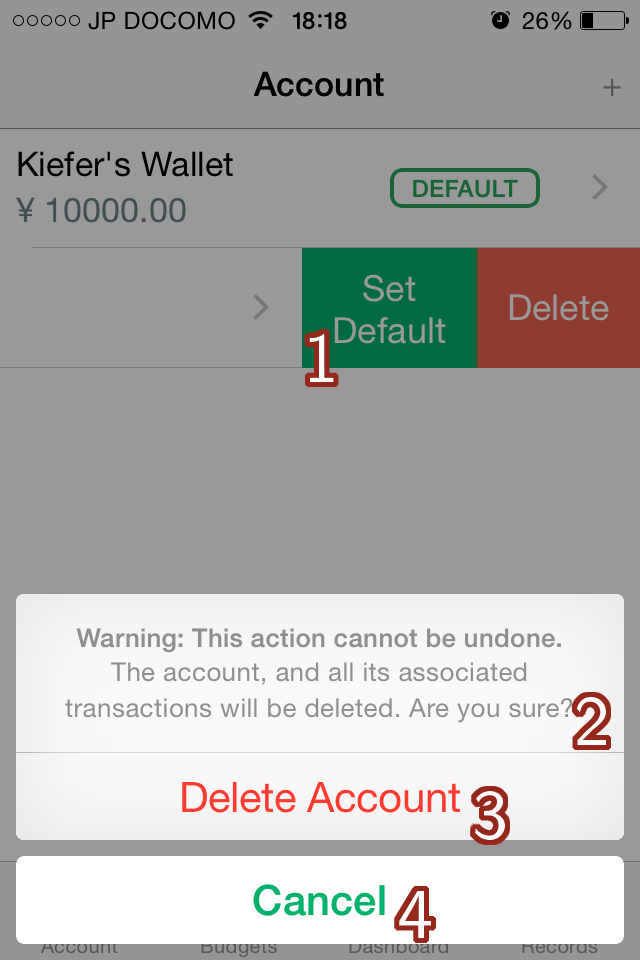
\includegraphics[scale=0.35]{ACC-0003-4}
  \caption{Deleting from the Account Display}
  \label{fig:delete-account-2}
\end{subfigure}
\caption{Account Deletion Screenshots}
\end{figure}


\screentable{
	\header{Screen Component}
    	{Type}
        {Description}
    \row{1. Cancellation Area}
    	{Dimmed black opacity}
        {
        Tap anywhere within the darkened area, and the alert controller will be dismissed.
        }  
    \row{2. Deletion Message}
    	{Alert Controller}
        {
        This alert controller is in the style of an action sheet. It displays the title and the message of the alert.\doublenewline
        
        Localization Keys: LABEL\_WARNING\_ DELETE\_ACCOUNT\_TITLE, LABEL\_ WARNING\_DELETE\_ACCOUNT\_ MESSAGE	
        }
        \row{3. Delete Alert Action}
    	{Alert Action}
        {
        Once tapped, this button will delete the selected account from the core data. \doublenewline
        
        Localization Key: BUTTON\_DELETE\_ACCOUNT
        }
    \row{4. Cancel Alert Action}
    	{Alert Action}
        {
        Once tapped, the alert controller will be dismissed. \doublenewline
        
        Localization Key: BUTTON\_CANCEL
        } 
}

\subsubsection{Use Cases}